\documentclass[14pt,a4paper,report]{report}
\usepackage[a4paper, mag=1000, left=2.5cm, right=1cm, top=2cm, bottom=2cm, headsep=0.7cm, footskip=1cm]{geometry}
\usepackage[utf8]{inputenc}
\usepackage[english,russian]{babel}
\usepackage{indentfirst}
\usepackage[dvipsnames]{xcolor}
\usepackage[colorlinks]{hyperref}
\usepackage{listings} 
\usepackage{fancyhdr}
\usepackage{caption}
\usepackage{amsmath}
\usepackage{latexsym}
\usepackage{graphicx}
\usepackage{amsmath}
\hypersetup{
	colorlinks = true,
	linkcolor  = black
}

\usepackage{titlesec}
\titleformat{\chapter}
{\Large\bfseries} % format
{}                % label
{0pt}             % sep
{\huge}           % before-code


\DeclareCaptionFont{white}{\color{white}} 

% Listing description
\usepackage{listings} 
\DeclareCaptionFormat{listing}{\colorbox{gray}{\parbox{\textwidth}{#1#2#3}}}
\captionsetup[lstlisting]{format=listing,labelfont=white,textfont=white}
\lstset{ 
	% Listing settings
	inputencoding = utf8,			
	extendedchars = \true, 
	keepspaces = true, 			  	 % Поддержка кириллицы и пробелов в комментариях
	language = Matlab,            	 	 % Язык программирования (для подсветки)
	basicstyle = \small\sffamily, 	 % Размер и начертание шрифта для подсветки кода
	numbers = left,               	 % Где поставить нумерацию строк (слева\справа)
	numberstyle = \tiny,          	 % Размер шрифта для номеров строк
	stepnumber = 1,               	 % Размер шага между двумя номерами строк
	numbersep = 5pt,              	 % Как далеко отстоят номера строк от подсвечиваемого кода
	backgroundcolor = \color{white}, % Цвет фона подсветки - используем \usepackage{color}
	showspaces = false,           	 % Показывать или нет пробелы специальными отступами
	showstringspaces = false,    	 % Показывать или нет пробелы в строках
	showtabs = false,           	 % Показывать или нет табуляцию в строках
	frame = single,              	 % Рисовать рамку вокруг кода
	tabsize = 2,                  	 % Размер табуляции по умолчанию равен 2 пробелам
	captionpos = t,             	 % Позиция заголовка вверху [t] или внизу [b] 
	breaklines = true,           	 % Автоматически переносить строки (да\нет)
	breakatwhitespace = false,   	 % Переносить строки только если есть пробел
	escapeinside = {\%*}{*)}      	 % Если нужно добавить комментарии в коде
}

\begin{document}
	
	\def\contentsname{Содержание}
	
	% Titlepage
	\begin{titlepage}
		\begin{center}
			\textsc{Санкт-Петербургский Политехнический 
				Университет Петра Великого\\[5mm]
				Кафедра компьютерных систем и программных технологий}
			
			\vfill
			
			\textbf{Отчёт по лабораторной работе №3\\[3mm]
				Курс: «Теория автоматического управления»\\[3mm]
				Тема: «Оптимизация качества системы»\\[35mm]
			}
		\end{center}
		
		\hfill
		\begin{minipage}{.5\textwidth}
			Выполнил студент:\\[2mm] 
			Раскин Андрей Романович\\
			Группа: 43501/3\\[5mm]
			
			Проверил:\\[2mm] 
			Нестеров Сергей Александрович
		\end{minipage}
		\vfill
		\begin{center}
			Санкт-Петербург\\ \the\year\ г.
		\end{center}
	\end{titlepage}
	
	% Contents
	\tableofcontents
	\clearpage
	
	\chapter{Лабораторная работа №3}
	
	\section{Цель работы}
	
	Научиться определять оптимальные критерии качества для замкнутой системы.
	
	\section{Программа работы}
	
	\begin{itemize}
		\item Определить область устойчивости
		\item Определить величину статической ошибки.
		\item Получить корневые критерии качества.
		\item Получить частотные критерии качества.
		\item Получить интегральные критерии качества.
		\item Промоделировать процессы в системе при оптимальных параметрах при наличии шума и без.
	\end{itemize}
	
	\section{Индивидуальное задание}
	
	$a_0=0.75,a_1=2,b_0=0,b_1=1,  y(0)=0, y'(0)=0, u=1(t)$
	\\
	$
	x''+2x'+0.75x=u'
	$
	
	
	\section{Ход работы}
	
	\subsection{Исходные данные замкнутой системы}
	
	Структура исследуемой системы с добавлением изодромного звена и шума:
	
%	\begin{figure}[h!]
%		\centering
%		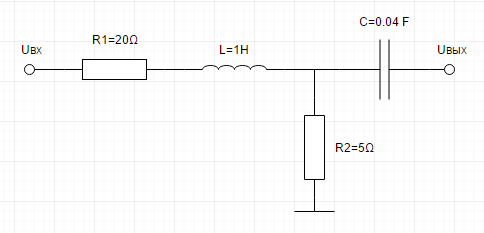
\includegraphics[scale = 0.70]{images/schema.png}
%		\caption{Структурная схема системы}
%		\label{image:1}
%	\end{figure}
	
	\clearpage
	
	Определим передаточную функцию разомкнутой системы:
	
	\begin{center}
		$W_p=\frac{B(p)}{C(p)}=\frac{kTp^2+kp}{p^3+2p^2+0.75p}$
	\end{center}
	
	Определим характеристический полином замкнутой системы:
	
	\begin{center}
		$D(p)=B(p)+C(p)=kTp^2+kp+p^3+2p^2+0.75p=p^3+(2+kT)p^2+(0.75+k)p$
	\end{center}
	
	Определим передаточную функцию замкнутой системы:
	
	\begin{center}
		$W_3=\frac{B(p)}{B(p)+C(p)}=\frac{B(p)}{D(p)}=\frac{kTp^2+kp}{p^3+(2+kT)p^2+(0.75+k)p}$
	\end{center}
	
	\subsection{Определение области устойчивости}
	
	Для выполнения необходимого условия устойчивости системы необходимо, чтобы коэффициенты характеристического полинома были положительны. Для этого должны выполняться следующие условия:
	
	\begin{equation*}
	\begin{cases}
	\text{$2+kT>0$} \\
	\text{$0.75+k>0$} \\
	\text{$T>0$}
	\end{cases}
	\Longrightarrow
	\begin{cases}
	\text{$kT>-2$} \\
	\text{$k>-0.75$} \\
	\text{$T>0$}
	\end{cases}
	\end{equation*}
	
	Так $T$ постоянная времени, то она не может быть отрицательной, поэтому результирующие условия устойчивости:
	
	\begin{equation*}
	\begin{cases}
	\text{$T>0$} \\
	\text{$k>0$}
	\end{cases}
	\end{equation*}
	
	Для определения достаточного условия устойчивости воспользуемся критерием Гурвица для системы третьего порядка:
	
	\begin{center}
		$a_2a_1-a_3a_0>0$ \\
		$(kT+2)(0.75+k)>0$ \\
	\end{center}
	
	Из неравенства очевидно, что для всех $k$ и $T$, удовлетворяющих достаточному условию, необходимое условие также соблюдается.
	
	\subsection{Статическая ошибка}
	
	Для данной системы статическая ошибка вычисляется следующим образом:
	
	\begin{center}
		$e=lim_{t\rightarrow\infty}\frac{1(t)}{1+W_p(t)}$
	\end{center}
	
	Так как система является астатической, то при $t\rightarrow\infty$ ошибка будет стремиться к нулю независимо от входного сигнала.
	
	\subsection{Корневые критерии качества}
	
	Данная группа критериев применяется для оценки качества системы по корням характеристического полинома:
	
	\begin{center}
		$D(p)=p^3+5(kT+5)p^2+5k(5T+1)p+25k$
	\end{center}
	
	\textbf{Оценка быстродействия} может производиться на основе величины:
	
	\begin{center}
		$\Omega=\sqrt[n]{|p_1\cdot...\cdot p_n|}$
	\end{center}
	
	Для данной системы существует три корня, которые легко находятся по теореме Виета:
	
	\begin{center}
		$\Omega=\sqrt[3]{|p_1\cdot p_2\cdot p_3|}=\sqrt[3]{|-a_3/a_0|}=\sqrt[3]{0.75+k}$
	\end{center}
	
	\textbf{Степень устойчивости} системы определяется как абсолютное значение реальной части корней, ближайших к мнимой оси корня (к нулю):
	
	\begin{center}
		$realPart = min(|Re(p_1)|, |Re(p_2)|, |Re(p_3)|)$
	\end{center}
	
	Таким образом, для получения оптимальных параметров $k$ и $T$, значение $realPart$ нужно минимизировать.
	
	\textbf{Колебательность системы} определяется мнимыми частями корней. Для нулевой колебательности все мнимые части коренй должны быть равны нулю:
	
	\begin{center}
		$imaginePart = (Im(p_1)=0\quad and\quad Im(p_2)=0\quad and\quad Im(p_3)=0)$
	\end{center}
	
	Таким образом, для получения оптимальных параметров $k$ и $T$, значение $imaginePart$ должно быть $True$.
	
	\subsection{Частотные критерии качества}
	
	Для оценки качества системы по частотным критериям представим передаточную функцию в частотном виде:
	
	\begin{center}
		$W_3(j\omega)=Re(\omega)+Im(\omega)j$  \linebreak \linebreak
		$Re(\omega)=\frac{-1.75k\omega^2+k\omega^4-2k^2T\omega^4-kT^2\omega^4}{Zn(\omega)}$ \linebreak \linebreak
		$Im(\omega)=\frac{2k\omega^3+k^2T\omega^3+kT\omega^5-0.75kT}{Zn(\omega)}$ \linebreak \linebreak
		$Zn(\omega)=\omega^4(2+kT)^2+(\omega(k+0.75)-\omega^3)^2$ \linebreak \linebreak
		$A(\omega)=\sqrt{Re^2(\omega)+Im^2(\omega)}$ \linebreak \linebreak
		$L(\omega)=20lg(A(\omega))$
	\end{center}
	
	\textbf{Показатель колебательности} определяется как отношение максимального модуля АЧХ к его значению при нулевой частоте:
	
	\begin{center}
		$\theta=\frac{max(A(\omega))}{A(0)}$
	\end{center}
	
	Так как значение АЧХ при нулевой частоте равно единице для любых значений $k$ и $T$:
	
	\begin{center}
		$\theta=max(A(\omega))$
	\end{center}
	
	Таким образом, для получения оптимальных параметров $k$ и $T$, значение $\theta$ нужно минимизировать. Однако, стоит отметить, что ниже единицы показатель колебательности быть не может, потому что при нулевой частоте он всегда равен единице (идеальный показатель колебательности).
	
	\textbf{Запас устойчивости по амплитуде} определяется следующим образом:
	
	\begin{center}
		$C(\theta)=\frac{\theta^2}{\theta^2-1}$
	\end{center}
	
	Тогда идеальный запас устойчивости по амплитуде равен бесконечности.
	
	\textbf{Запас устойчивости по фазе} определяется следующим образом:
	
	\begin{center}
		$\mu(\theta)=arccos(1-\frac{\theta^2}{2})$
	\end{center}
	
	Тогда идеальный запас устойчивости по фазе равен $\pi/3$.
	
	\subsection{Интегральные критерии качества}
	
	Воспользуемся квадратичным критерием качества:
	
	\begin{center}
		$I=\int_{0}^{\infty}x^2(t)dt$
	\end{center}
	
	Для данной системы $x^2(t)=(h(t)-1(t))^2$, где $h(t)$ - переходная характеристика замкнутой системы, а $1(t)$ - входное воздействие:
	
	\begin{center}
		$I=\int_{0}^{\infty}(h(t)-1(t))^2dt$
	\end{center}
	
	Таким образом, для получения оптимальных параметров $k$ и $T$, значение $I$  нужно минимизировать.
	
	\subsection{Получение оптимальных критериев качества}
	
	Воспользуемся средой \emph{Matlab} для поиска оптимальных параметров $k$ и $T$. Все вышеперечисленные условия должны по возможности выполняться.
	
%	\lstinputlisting{listings/script.m}
	
	Данный скрипт находит оптимальные значения $k$ и $T$, соответствующие вышеперечисленным условиям, после чего рассчитывает критерии качества, рисует графики переходной характеристики с шумом и без.
	
	В ходе исследования было выяснено, что оптимальное значение $k=0.2$. Меньшие и большие значения $k$ всегда выдают неоптимальные критерии качества.
	
	Однако, оптимальное значение для $T$ получить не удалось, потому что все критерии качества строго улучшались с увеличением параметра $T$. Таким образом, чем больше значение $T$, тем качественнее система. Выясним, как будет вести себя система при наличии шума. 
	
	\subsubsection{Моделирование системы при k=0.2 и T=10}
	
	Cтатическая ошибка:
	
	\begin{center}
		$e=0$
	\end{center}
	
	Оценка быстродействия:
	
	\begin{center}
		$\Omega=\sqrt[3]{5}$
	\end{center}
	
	Корни характеристического уравнения:
	
	\begin{equation*}
	\begin{cases}
	\text{$p_1=-33.481218271995985$} \\
	\text{$p_2=-1.413101065200161$} \\
	\text{$p_3=-0.105680662803830$}
	\end{cases}
	\end{equation*}
	
	Степень устойчивости:
	
	\begin{center}
		$min(|Re(p_1)|, |Re(p_2)|, |Re(p_3)|) = 0.105680662803830$
	\end{center}
	
	Колебательность системы:
	
	\begin{equation*}
	\begin{cases}
	\text{$Im(p_1)=0$} \\
	\text{$Im(p_2)=0$} \\
	\text{$Im(p_3)=0$}
	\end{cases}
	\end{equation*}
	
	Показатель колебательности:
	
	\begin{center}
		$\theta=1$
	\end{center}
	
	
	
	Запас устойчивости по амплитуде:
	
	\begin{center}
		$C(\theta)=\infty$
	\end{center}
	
	Запас устойчивости по фазе:
	
	\begin{center}
		$\mu(\theta)=\frac{\pi}{3}$
	\end{center}
	
	Полоса пропускания:
	
	\begin{center}
		$0\leq\omega\leq0.0706403255$
	\end{center}
	
	Квадратичный критерий качества:
	
	\begin{center}
		$I=\int_{0}^{\infty}(h(t)-1(t))^2dt=0.1898876404$
	\end{center}
	
	\clearpage
	
	Диаграмма боде:
	
	\begin{figure}[h!]
		\centering
		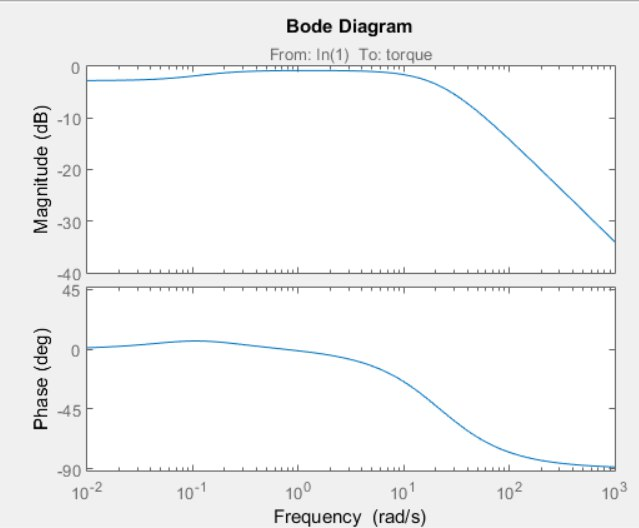
\includegraphics[scale = 0.53]{images/bode10.jpg}
		\caption{Диаграмма боде для k=0.2 и T=10}
		\label{image:2}
	\end{figure}
	
	Шум:
	
	\begin{figure}[h!]
		\centering
		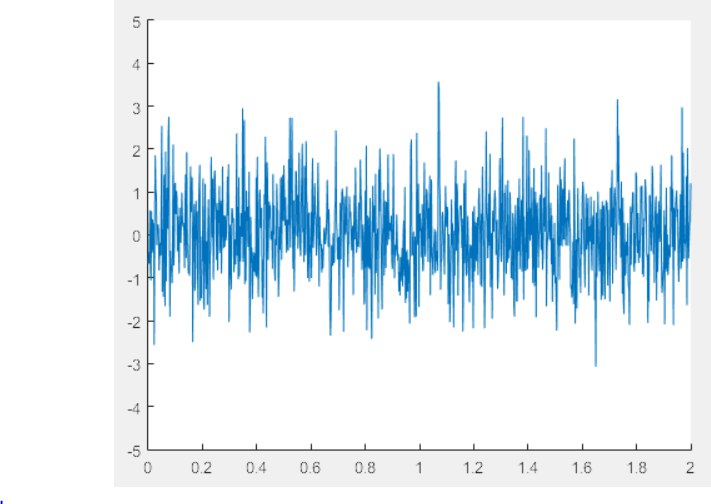
\includegraphics[scale = 0.53]{images/noice.jpg}
		\caption{Шум, накладываемый на переходную характеристику}
		\label{image:3}
	\end{figure}
	
	\clearpage
	
	Переходная характеристика без наложения шума:
	
	\begin{figure}[h!]
		\centering
		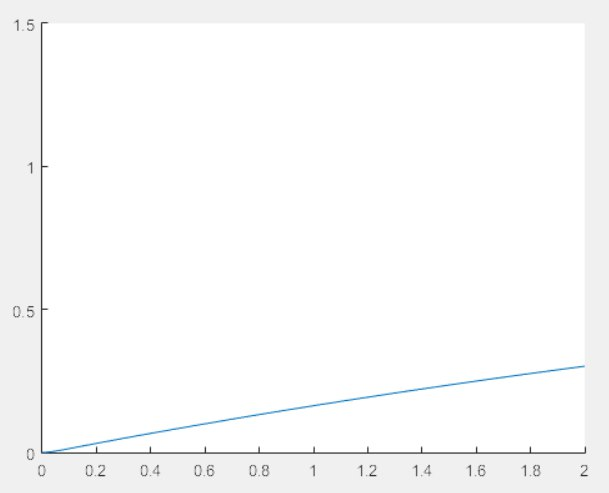
\includegraphics[scale = 0.55]{images/step10.jpg}
		\caption{Переходная характеристика без наложения шума для k=0.2 и T=10}
		\label{image:4}
	\end{figure}
	
	Переходная характеристика с наложением шума:
	
	\begin{figure}[h!]
		\centering
		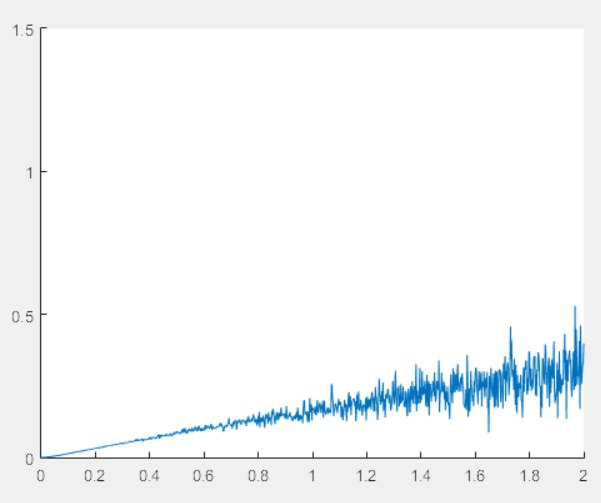
\includegraphics[scale = 0.55]{images/stepnoice10.jpg}
		\caption{Переходная характеристика с наложением шума для k=0.2 и T=10}
		\label{image:5}
	\end{figure}

	
	\section{Вывод}
	
	При использовании изодромного звена в качестве управляющего устройства, оптимальные параметры не удалось установить однозначным образом. Как оказалось, параметр $T$ улучшает качественнные характеристики системы, поэтому при конструировании управляющего устройства следует выбирать максимально возможное $T$. Из эксперимента можно заметить, что при больших значениях $T$ улучшается степень устойчивости, увеличивается полоса пропускания, уменьшается воздействие шума, а также увеличивается скорость установления переходной характеристики.
	
	Однако, параметр $k$ изодромного звена был получен однозначно: $k=0.2$. Любые отклонения от этого значения ухудшают качественные характеристики системы и вносят элемент колебательности.
	
	Стоит отметить, что описанные правила для выбора $k$ и $T$ справедливы для только ОУ с конкретной переходной характеристикой, в то время как для других ОУ эти значения должны рассчитываться отдельно.
	
	
	
	
\end{document}